%% Example data sheet
%% Feel free to modify and use this file for any purpose, under
%% either the LaTeX Project Public License or under public domain.

% Options here are passed to the article class.
% Most common options: 10pt, 11pt, 12pt
\documentclass[10pt]{datasheet}

% Input encoding and typographical rules for English language
\usepackage[utf8]{inputenc}
\usepackage[english]{babel}
\usepackage[english]{isodate}

% tikz is used to draw images in this example, but you can
% also use \includegraphics{}.
\usepackage{tikz}
\usepackage{pgfplots}
\usepackage{circuitikz}
\usetikzlibrary{calc}

% These define global texts that are used in headers and titles.
\title{MIPS CPU Data-sheet}
\date{December 2020}

\begin{document}
\maketitle

\section{Overall Architecture}
\smallbreak

\section{Design Decisions}
Overall our design Incorporated a number of 
\textbf{Five stage pipeline} this choice enabled a ...

\textbf{Branch prediction} this choice was a key to the low...

\textbf{Caching} this choice was ...


\smallbreak


% Switch to next column
\vfill\break

\section{Architecture Diagram}
\smallbreak
\begin{figure}[h]
    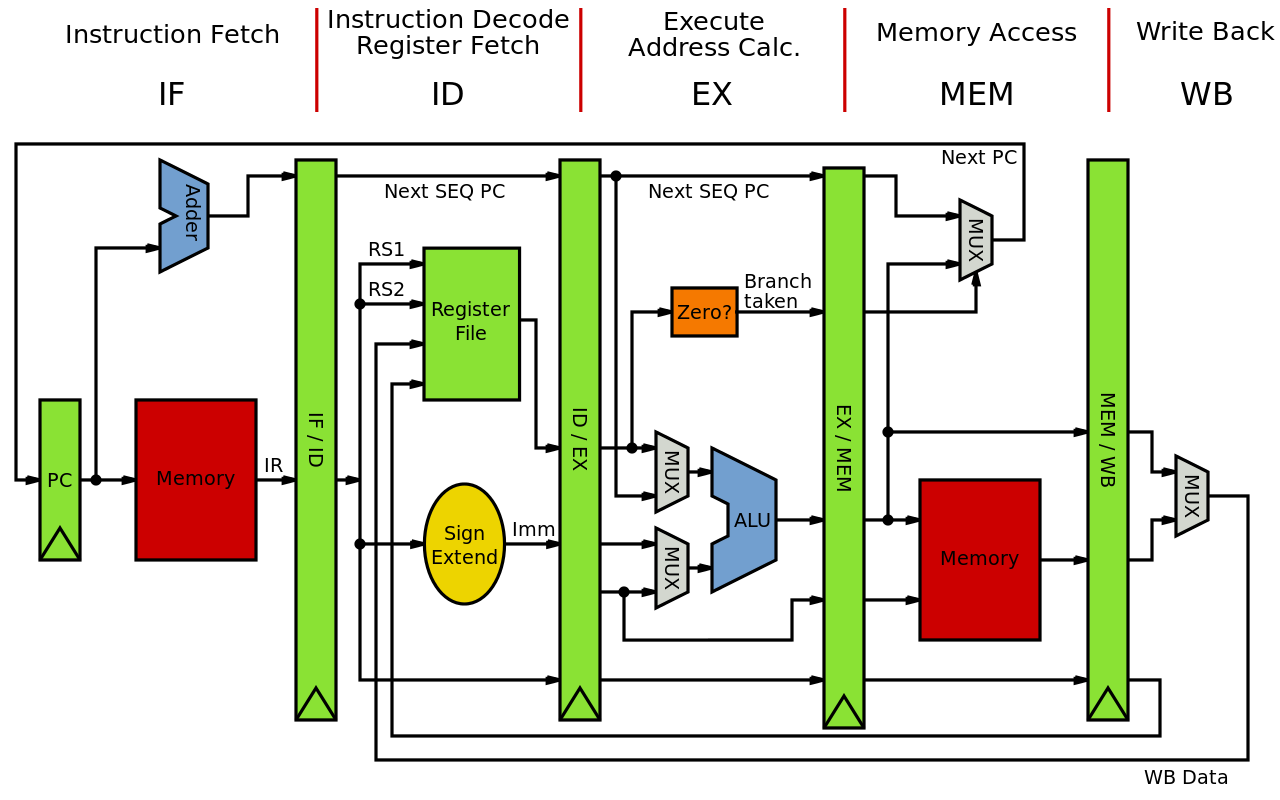
\includegraphics[scale=0.2]{MIPS_Architecture_(Pipelined).svg.png}
    \captionsetup{justification=centering}
    \caption{Mips Pipelined design (Place Holder)}
\end{figure}

Comments on said diagram


% For wide tables, a single column layout is better. It can be switched
% page-by-page.
\newpage

\onecolumn

\section{Design}

orem ipsum dolor sit amet, consectetur adipiscing elit. Fusce ultricies lorem sapien. Nullam sollicitudin molestie arcu, vitae commodo ligula tempor a. Vivamus et commodo tortor, eu elementum nisl. Maecenas bibendum urna eget nibh pharetra, et hendrerit purus cursus. Pellentesque habitant morbi tristique senectus et netus et malesuada fames ac turpis egestas. Duis ligula lectus, vehicula vitae quam ac, feugiat congue urna. Nullam eget rutrum enim. Nullam vitae hendrerit erat, id placerat velit. Fusce congue tellus lorem, vel porta mauris gravida molestie. Proin dignissim tellus sit amet nisi blandit rutrum. Suspendisse potenti. Nunc sed libero ut orci eleifend porta sit amet eu massa. Ut quis ante tellus. Sed id tempor libero, ut imperdiet lorem.

Vivamus ut libero diam. Proin ac placerat metus. Aliquam et blandit lectus. Donec elementum nisi ut felis feugiat euismod. Integer sagittis blandit tempus. Nam a arcu pharetra, lacinia ante eu, imperdiet nunc. Class aptent taciti sociosqu ad litora torquent per conubia nostra, per inceptos himenaeos. Suspendisse ex ante, finibus nec est in, bibendum ornare dui. Pellentesque habitant morbi tristique senectus et netus et malesuada fames ac turpis egestas.

Praesent et odio massa. Pellentesque tempus egestas commodo. Proin odio odio, lacinia consequat fermentum eget, porta eget elit. Curabitur lacinia, nisi in bibendum egestas, magna velit molestie lectus, at congue erat leo sed nisi. Aenean quis ipsum venenatis, faucibus leo sit amet, porttitor magna. Morbi semper, sapien vel pellentesque euismod, urna dui dapibus mi, ut commodo quam libero non massa. In eleifend at enim quis interdum. Aliquam a est mi. Nam neque arcu, pharetra nec finibus sit amet, gravida nec lorem. Donec sodales dolor consectetur velit tempus venenatis. Aenean bibendum nibh nunc, id auctor dolor molestie a. Vestibulum quis mi facilisis, dapibus lectus vel, molestie massa.

Orci varius natoque penatibus et magnis dis parturient montes, nascetur ridiculus mus. Fusce varius tristique leo vitae laoreet. Sed et hendrerit orci, non congue augue. Maecenas vitae maximus tellus. Curabitur mauris nulla, volutpat a finibus id, semper ac ipsum. Nulla sodales, quam id pellentesque efficitur, elit lectus scelerisque leo, mattis euismod sem augue a elit. Suspendisse dictum pulvinar dolor vel efficitur. Ut rutrum id mi eu aliquet. Donec accumsan nulla diam, at ornare ex dignissim eu. Nam ac urna a risus lobortis eleifend. Suspendisse vitae ullamcorper ligula. Sed iaculis, felis vel bibendum posuere, massa sem rutrum lectus, eget malesuada urna enim sed neque. Class aptent taciti sociosqu ad litora torquent per conubia nostra, per inceptos himenaeos. Praesent volutpat egestas tempus.



\begin{figure}[h]
    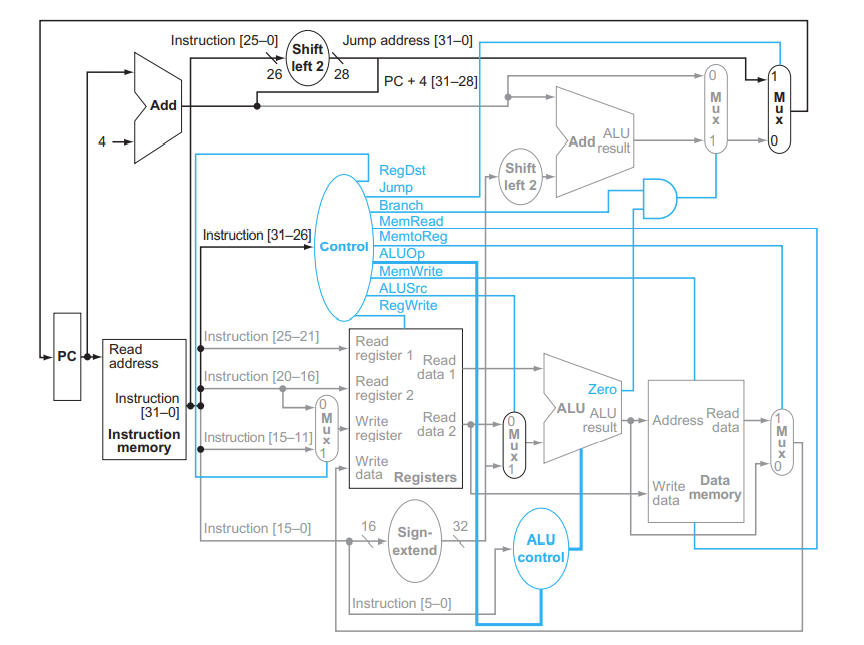
\includegraphics[scale=0.8]{Assets/examplearch.PNG}
    \centering
    \captionsetup{justification=centering}
    \caption{Exemplar Architecture}
\end{figure}


\newpage

\twocolumn

\section{Testing Approach}
\smallbreak
Testing was performed by two separate methodologies, one methodology tested the full architecture from ground up focusing on architecture robustness whilst a second tested for functional correctness using CPU I/O (as a third party would). This distinction ensured the testing was not designed to solely evaluate our architecture but could also be used on similar MIPS architectures. Further it prevented any framing or confirmation bias in evaluation of results.
\smallbreak

Each component varies in functionality and make up so testing was tailored for each component / block , the table highlights the test strategy used on each.

\begin{figure}[h]
    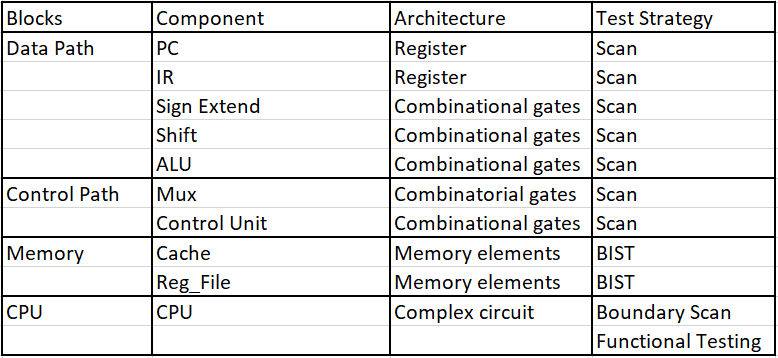
\includegraphics[scale=0.7]{Assets/Strategy.PNG}
    \captionsetup{justification=centering}
    \caption{Test Strategy table}
\end{figure}

\smallbreak


\textbf{Methodology one} (Robustness Testing): Performed all logic scan , BIST and boundary scan testing through the development of our architecture. This testing occurred in an order determined by the component hierarchy. Testing begins at each bottom component and moves up the hierarchy, testing intermediate circuity as it continues. 
\smallbreak

\begin{figure}[h]
    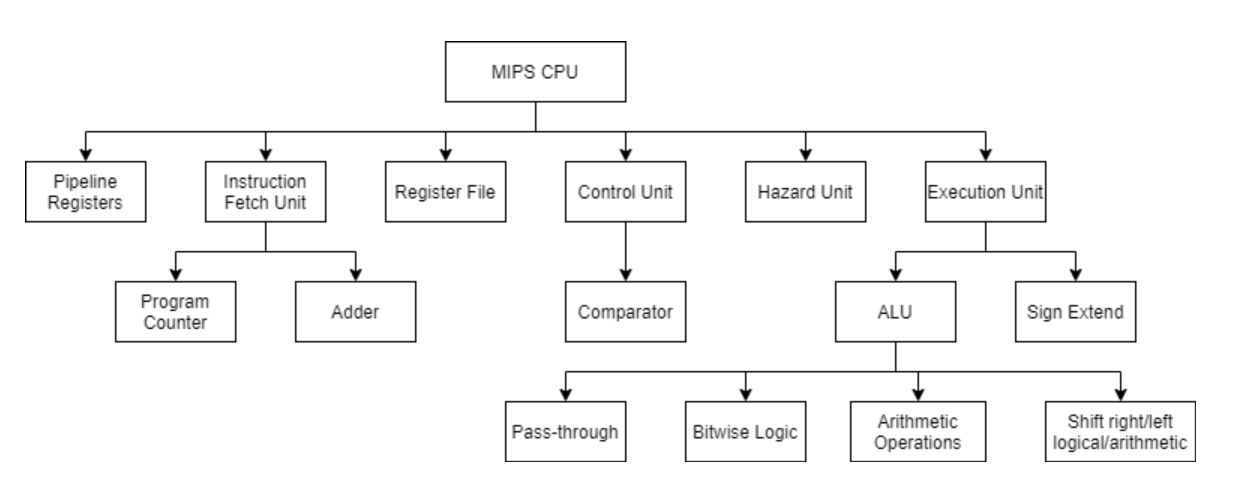
\includegraphics[scale=0.45]{Assets/hierarchy2.png}
    \captionsetup{justification=centering}
    \caption{CPU Component Hierarchy}
\end{figure}

\smallbreak

Component testing method:

1. Identify inputs, outputs and intended behaviour

2. Using verilator write cpp code, feeding the module with different inputs and checking outputs manually or automatically.
Manual: values chosen by hand to see how the module handles certain edge cases.Automatic: values chosen 'randomly' (on a set increment or by multiplying increments).

\vfill\break

3. If a test case fails, log information usually inputs, expected value, returned value and any other outputs from the module.

 



\textbf{Methodology Two} (Functional Testing): Utilises a virtual RAM to control inputs to the CPU and as such, tests individual and combinations of instructions. Again it follows a ground up approach testing the least logically and architecturally complex instructions first. R-Type instructions (aside from 3 shift instructions) only use registers in their operation so were tested first. Followed by J-Type then I-Type. After this programs containing edge cases are tested and then exemplar programs designed to complex functionality such as recursion.
\begin{figure}[h]
    \centering
    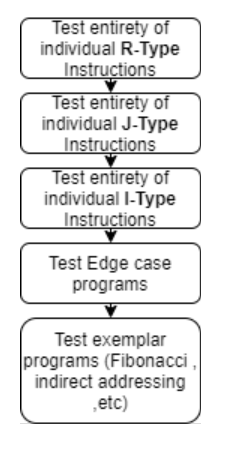
\includegraphics[scale=0.7]{Assets/functflow.PNG}
    \captionsetup{justification=centering}
    \caption{Functionality testing flowchart}
\end{figure}



\section{Testing Flow}
Maybe not needed but can be used to fill up to hit more design points on functiona testing?
\smallbreak



\onecolumn

\section{Area and timing summary}
\smallbreak

\begin{table}[h]
\caption{Summary CPU Specifications}
\begin{tabularx}{\textwidth}{l | c | c c c | c | X}
    \thickhline
    \textbf{Parameter} & \textbf{Symbol} & \textbf{Min.} & \textbf{Typ.} & \textbf{Max.} &
    \textbf{Unit} & \textbf{Conditions} \\
    \hline
    Page width  & $p_w$ & 20.9 & 21.0 & 21.1 & cm & \multirow{2}{*}{Standard A4 paper} \\
    Page height & $p_h$ & 29.6 & 29.7 & 29.8 & cm &  \\
    \hline
    Insulation voltage & $E_{max}$\footnotemark[1] & & 1 & & kV & \\
    \thickhline
\end{tabularx}
\footnotetext[1]{Based on characterization data, not tested in production.}
\end{table}

\textbf{Note:} All measurements taken above were performed in the Cyclone IV E Auto Quartus

\end{document}


